% ---------------------------------------------------------------
\section{Empirical Results: National Research Evaluation in Australia}
\label{sec:results}
% ---------------------------------------------------------------

\subsection{Institutional Profiles of Australian Higher Education Providers}

Applying the bipartite spectral ranking model across all 42 Australian Higher Education Providers (HEPs) provides a comprehensive, size-independent mapping of Australian university research influence. 

Figure~\ref{fig:hep_heatmap} displays the full influence heatmap of Australian universities across all 26 OpenAlex disciplines for the 2020--2024 window, while Table~\ref{tab:hep_summary} reports institutional prestige scores ($v_I$) aggregated into the five canonical AREA5 broad disciplines.

\begin{figure}[htbp]
\centering
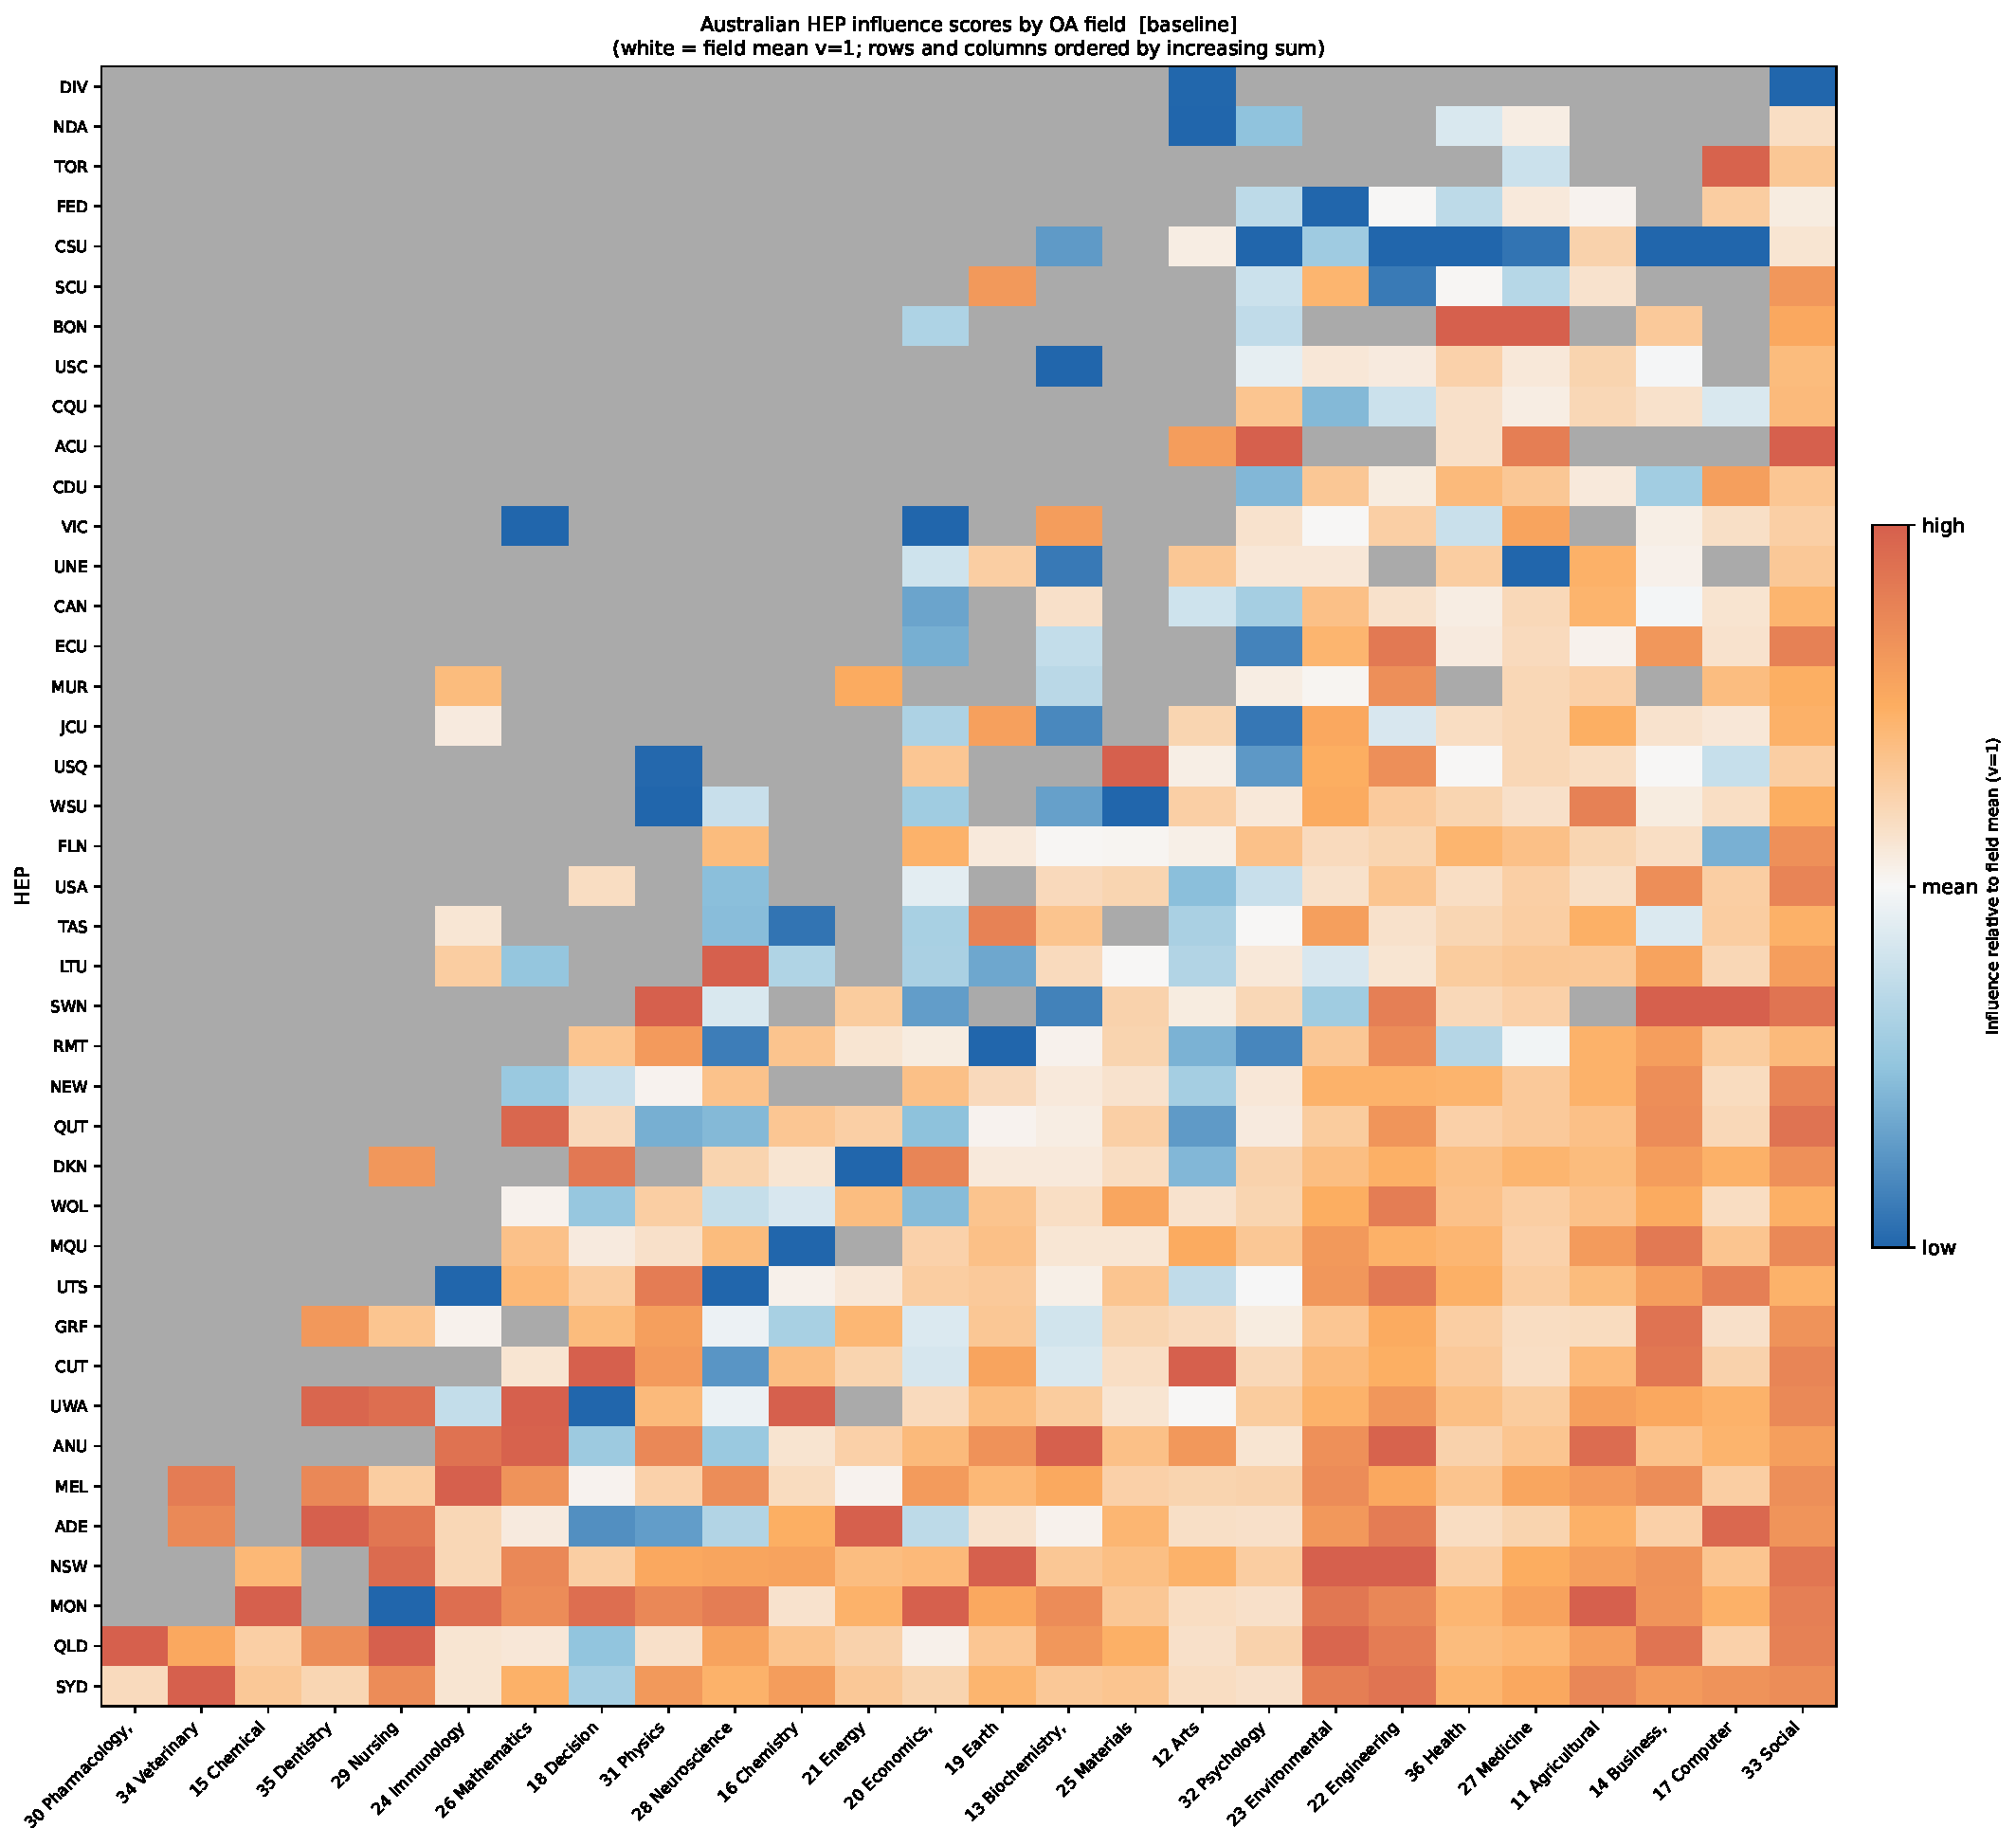
\includegraphics[width=\textwidth]{figures/fig2_hep_heatmap_fields.pdf}
\caption{Heatmap of Australian Higher Education Provider research influence scores ($v_I$) across 26 disciplines (2020--2024 census window). Cell colors range from blue ($v_I < 1.0$, below global mean) through white ($v_I = 1.0$, world average) to orange/red ($v_I > 1.0$, high research intensity). Institutions and disciplines are clustered by total influence.}
\label{fig:hep_heatmap}
\end{figure}

\begin{table}[htbp]
\centering
\small
\caption{Institutional Influence Scores ($v_I$) for Leading Australian Universities across the Five Broad Disciplines (World Average = 1.0).}
\label{tab:hep_summary}
\begin{tabularx}{\textwidth}{l >{\raggedright\arraybackslash}X c cccccc}
\toprule
\textbf{Code} & \textbf{Institution} & \textbf{Group} & \textbf{MCS} & \textbf{PSE} & \textbf{LES} & \textbf{BHS} & \textbf{SSH} & \textbf{Mean $v_I$} \\
\midrule
MON & Monash University & Go8 & 2.00 & 1.86 & 2.03 & 1.79 & 2.35 & \textbf{2.01} \\
SYD & University of Sydney & Go8 & 2.35 & 1.96 & 1.70 & 1.70 & 2.21 & \textbf{1.98} \\
SWN & Swinburne University of Technology & Non & 3.20 & 1.89 & 1.11 & 1.40 & 2.12 & \textbf{1.94} \\
ADE & University of Adelaide & Go8 & 2.92 & 1.95 & 1.38 & 1.38 & 1.96 & \textbf{1.92} \\
NSW & University of New South Wales & Go8 & 1.70 & 1.99 & 1.78 & 1.68 & 2.40 & \textbf{1.91} \\
UTS & University of Technology Sydney & ATN & 2.80 & 1.99 & 1.47 & 1.32 & 1.89 & \textbf{1.89} \\
ACU & Australian Catholic University & Non & 1.12 & -- & 1.55 & 1.86 & 2.92 & \textbf{1.86} \\
QLD & University of Queensland & Go8 & 1.68 & 1.96 & 1.76 & 1.58 & 2.24 & \textbf{1.85} \\
ANU & Australian National University & Go8 & 2.03 & 1.79 & 1.93 & 1.43 & 1.97 & \textbf{1.83} \\
MEL & University of Melbourne & Go8 & 1.66 & 1.61 & 1.76 & 1.73 & 2.16 & \textbf{1.79} \\
DKN & Deakin University & ATN & 2.08 & 1.45 & 1.33 & 1.56 & 2.19 & \textbf{1.72} \\
UWA & University of Western Australia & Go8 & 1.84 & 1.83 & 1.38 & 1.39 & 2.11 & \textbf{1.71} \\
TOR & Torrens University Australia & Non & 3.15 & -- & -- & 0.78 & 1.11 & \textbf{1.68} \\
MQU & Macquarie University & Non & 1.74 & 1.47 & 1.43 & 1.40 & 2.22 & \textbf{1.65} \\
QUT & Queensland University of Technology & Non & 1.53 & 1.69 & 1.39 & 1.39 & 2.09 & \textbf{1.62} \\
BON & Bond University & Non & -- & 1.15 & 0.49 & 2.30 & 2.43 & \textbf{1.59} \\
WOL & University of Wollongong & Non & 1.38 & 1.75 & 1.43 & 1.34 & 2.02 & \textbf{1.59} \\
CUT & Curtin University & ATN & 1.46 & 1.62 & 1.41 & 1.22 & 2.14 & \textbf{1.57} \\
NEW & University of Newcastle & Non & 1.32 & 1.54 & 1.42 & 1.40 & 2.16 & \textbf{1.57} \\
USA & University of South Australia & ATN & 1.59 & 1.60 & 1.36 & 1.37 & 1.88 & \textbf{1.56} \\
MUR & Murdoch University & IRU & 1.85 & 1.82 & 0.96 & 1.21 & 1.65 & \textbf{1.50} \\
ECU & Edith Cowan University & Non & 1.29 & 1.96 & 1.33 & 1.14 & 1.77 & \textbf{1.50} \\
RMT & RMIT University & ATN & 1.64 & 1.73 & 1.35 & 1.03 & 1.65 & \textbf{1.48} \\
CDU & Charles Darwin University & IRU & 2.32 & 1.01 & 1.21 & 1.49 & 1.37 & \textbf{1.48} \\
GRF & Griffith University & IRU & 1.35 & 1.62 & 1.25 & 1.21 & 1.92 & \textbf{1.47} \\
\bottomrule
\end{tabularx}
\end{table}


Several pivotal empirical findings emerge from this national analysis:

\begin{enumerate}
    \item \textbf{Comprehensive Excellence among the Group of Eight (Go8)}:
    All eight Go8 members achieve overall mean influence scores between $1.71$ and $2.01$, indicating that their research output attracts 70\% to 100\% more global prestige per unit than the world baseline. Monash University (MON, mean $v_I = 2.01$), the University of Sydney (SYD, $v_I = 1.98$), UNSW Sydney (NSW, $v_I = 1.91$), and the University of Adelaide (ADE, $v_I = 1.92$) exhibit broad-based intensity exceeding $1.6$ across all five macro-disciplines.
    
    \item \textbf{Specialized High-Intensity Clusters in the ATN and Non-Go8 Universities}:
    Crucially, the size-independent intensity metric $v_I$ reveals world-leading excellence outside the traditional Go8 establishment. Swinburne University of Technology (SWN) and the University of Technology Sydney (UTS) record extraordinary intensity in \textit{Mathematics, Computing and Information Sciences} (MCS $v_I = 3.21$ and $2.80$, respectively), outperforming all comprehensive universities in computing. Both institutions also demonstrate premier status in \textit{Physical Sciences and Engineering} (PSE $v_I = 1.89$ and $1.99$).
    
    \item \textbf{High-Intensity Niche Performers}:
    Australian Catholic University (ACU) provides a compelling demonstration of the metric's utility. Despite possessing a modest total volume of publications, ACU achieves the nation's highest institutional score in \textit{Social Sciences, Humanities and Business} (SSH $v_I = 2.92$) and strong biomedical/nursing performance (BHS $v_I = 1.86$), driving a mean institutional intensity of $1.86$. Under traditional volume-dependent metrics, ACU's distinctive research quality is frequently obscured.
    
    \item \textbf{Mission-Specific Strengths in Regional Universities}:
    Universities in the Regional Universities Network (RUN) and Innovative Research Universities (IRU) display targeted disciplinary excellence. For example, Deakin University (DKN, mean $v_I = 1.72$) achieves world-class status in computing (MCS $v_I = 2.08$) and social sciences (SSH $v_I = 2.20$), while Charles Darwin University (CDU) demonstrates localized environmental research strength.
\end{enumerate}

\subsection{Cross-Country Comparative Context}

To demonstrate that the bipartite spectral framework functions robustly across distinct national governance structures, Figure~\ref{fig:country_heatmap} illustrates national institutional profiles for Australia alongside the United Kingdom and the United States.

\begin{figure}[htbp]
\centering
\begin{minipage}{0.48\textwidth}
    \centering
    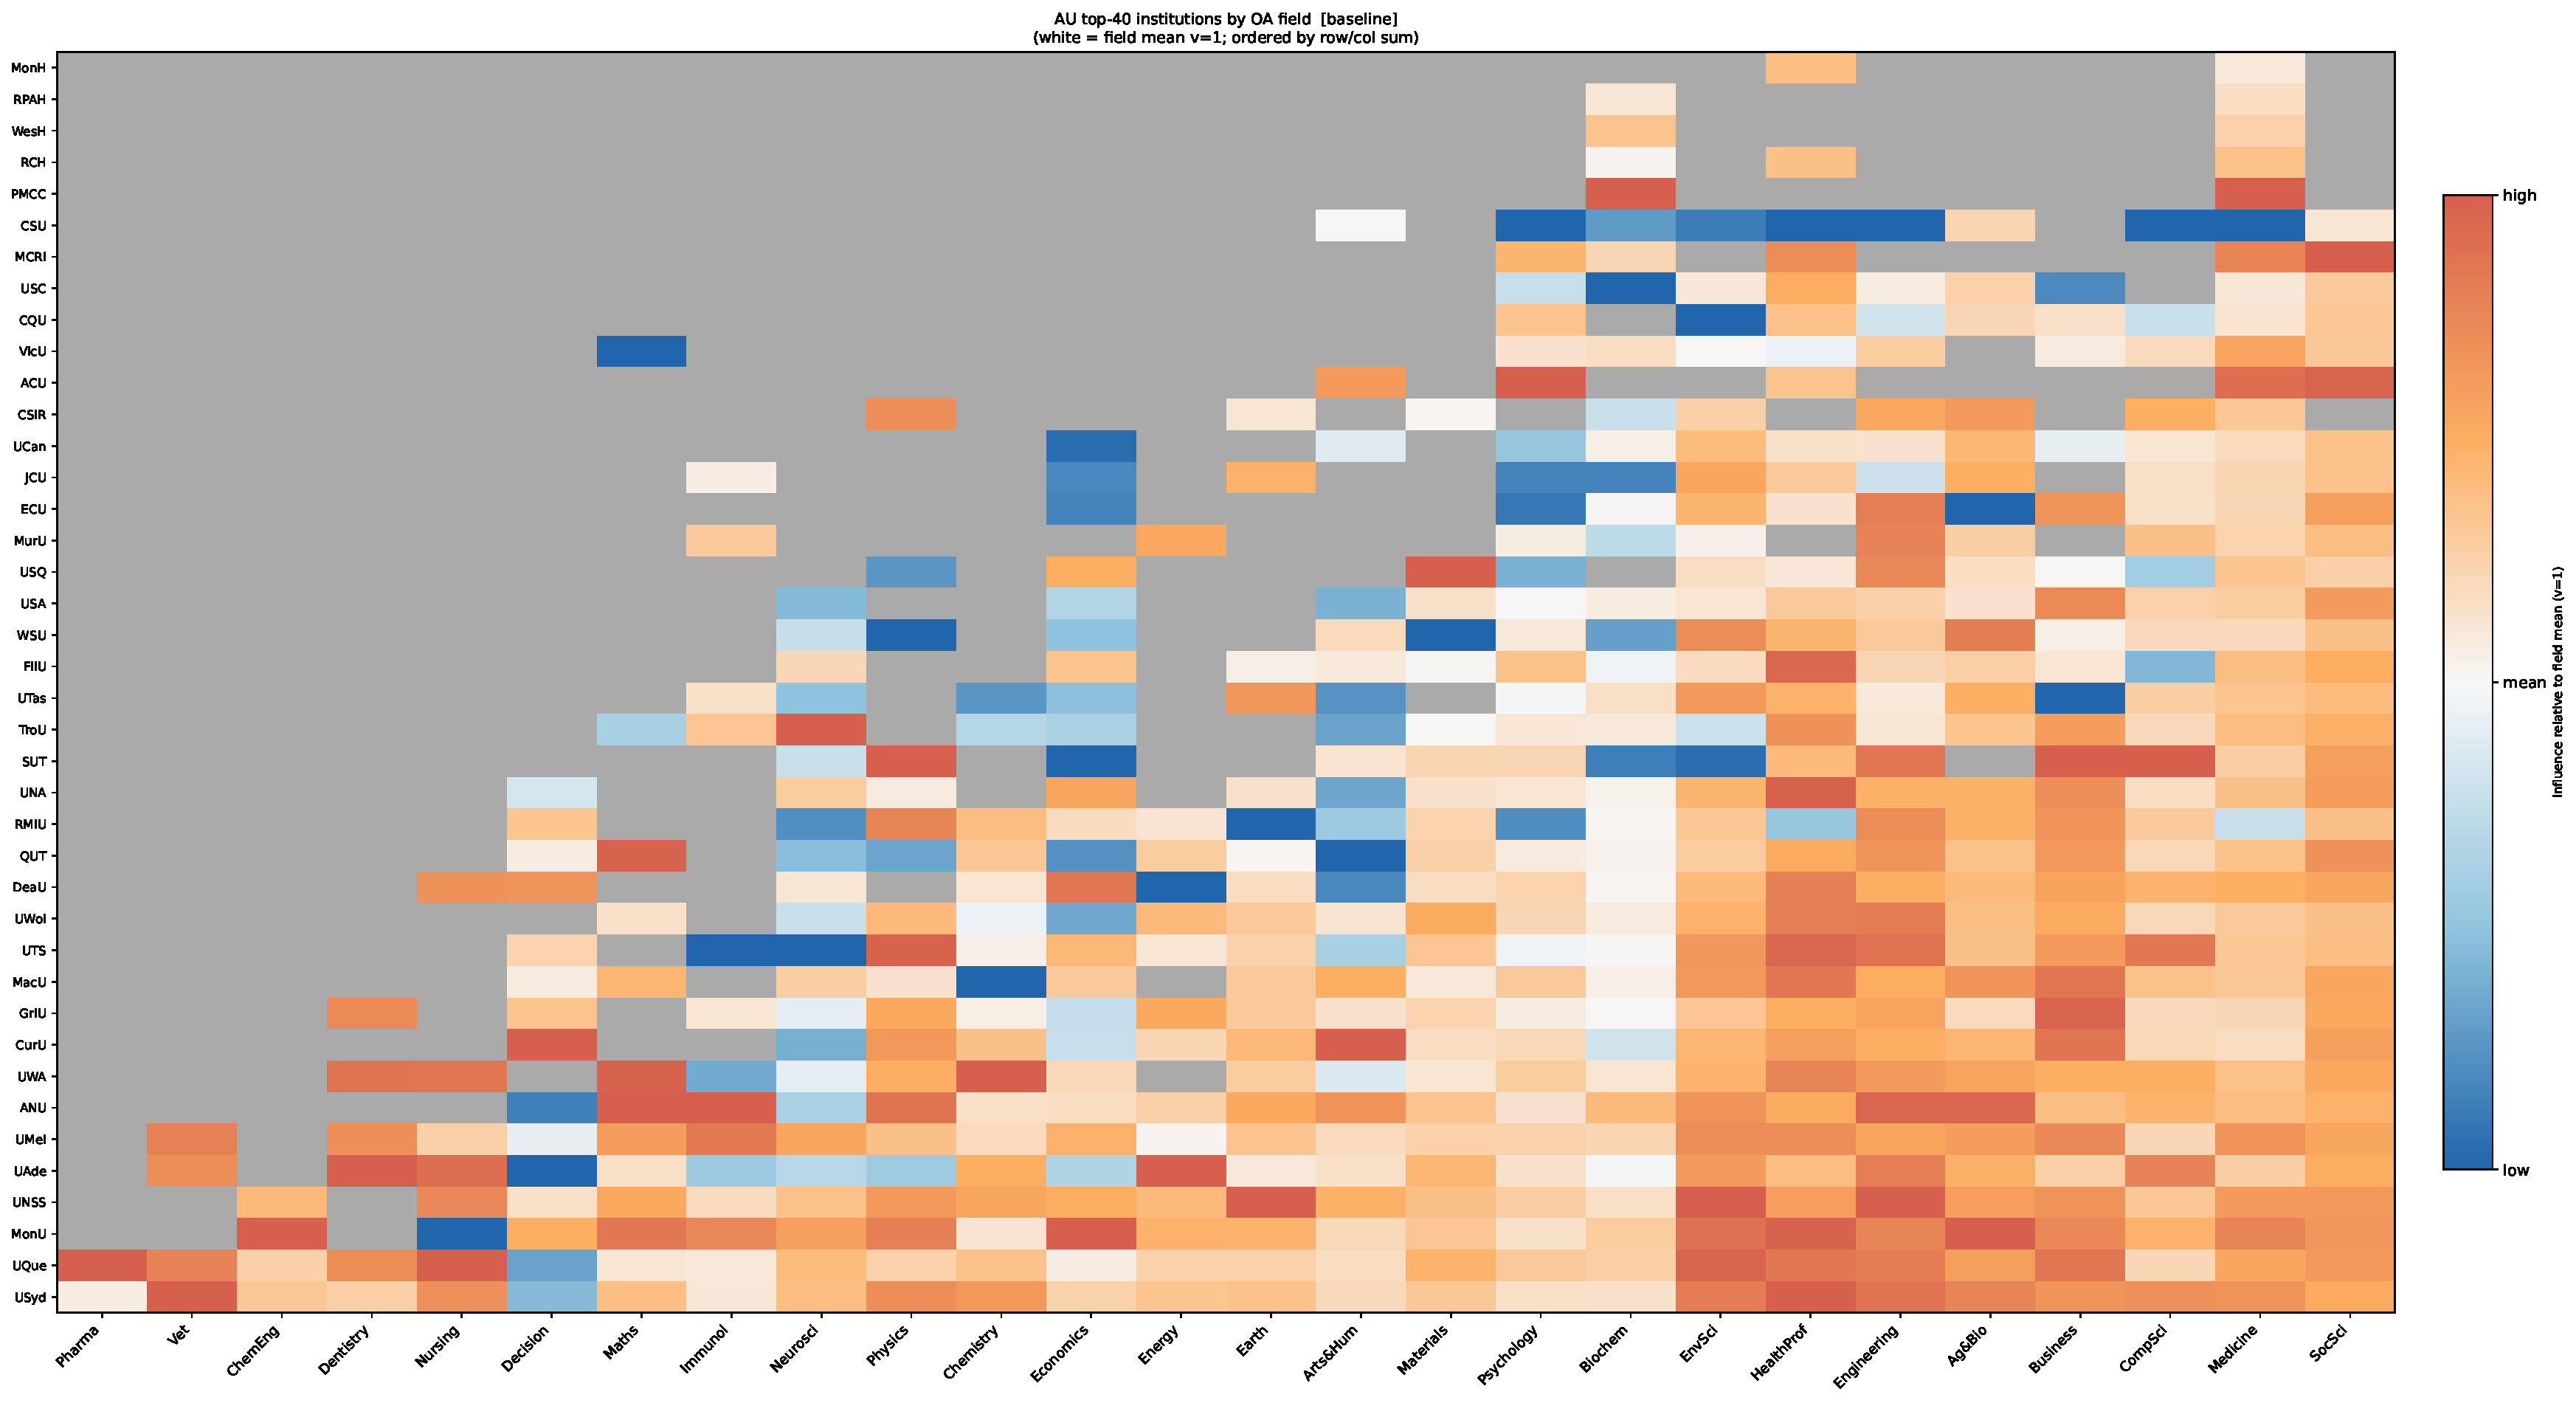
\includegraphics[width=\textwidth]{figures/fig3_country_heatmap_au.pdf}
    \caption*{(a) Australia (AU)}
\end{minipage}\hfill
\begin{minipage}{0.48\textwidth}
    \centering
    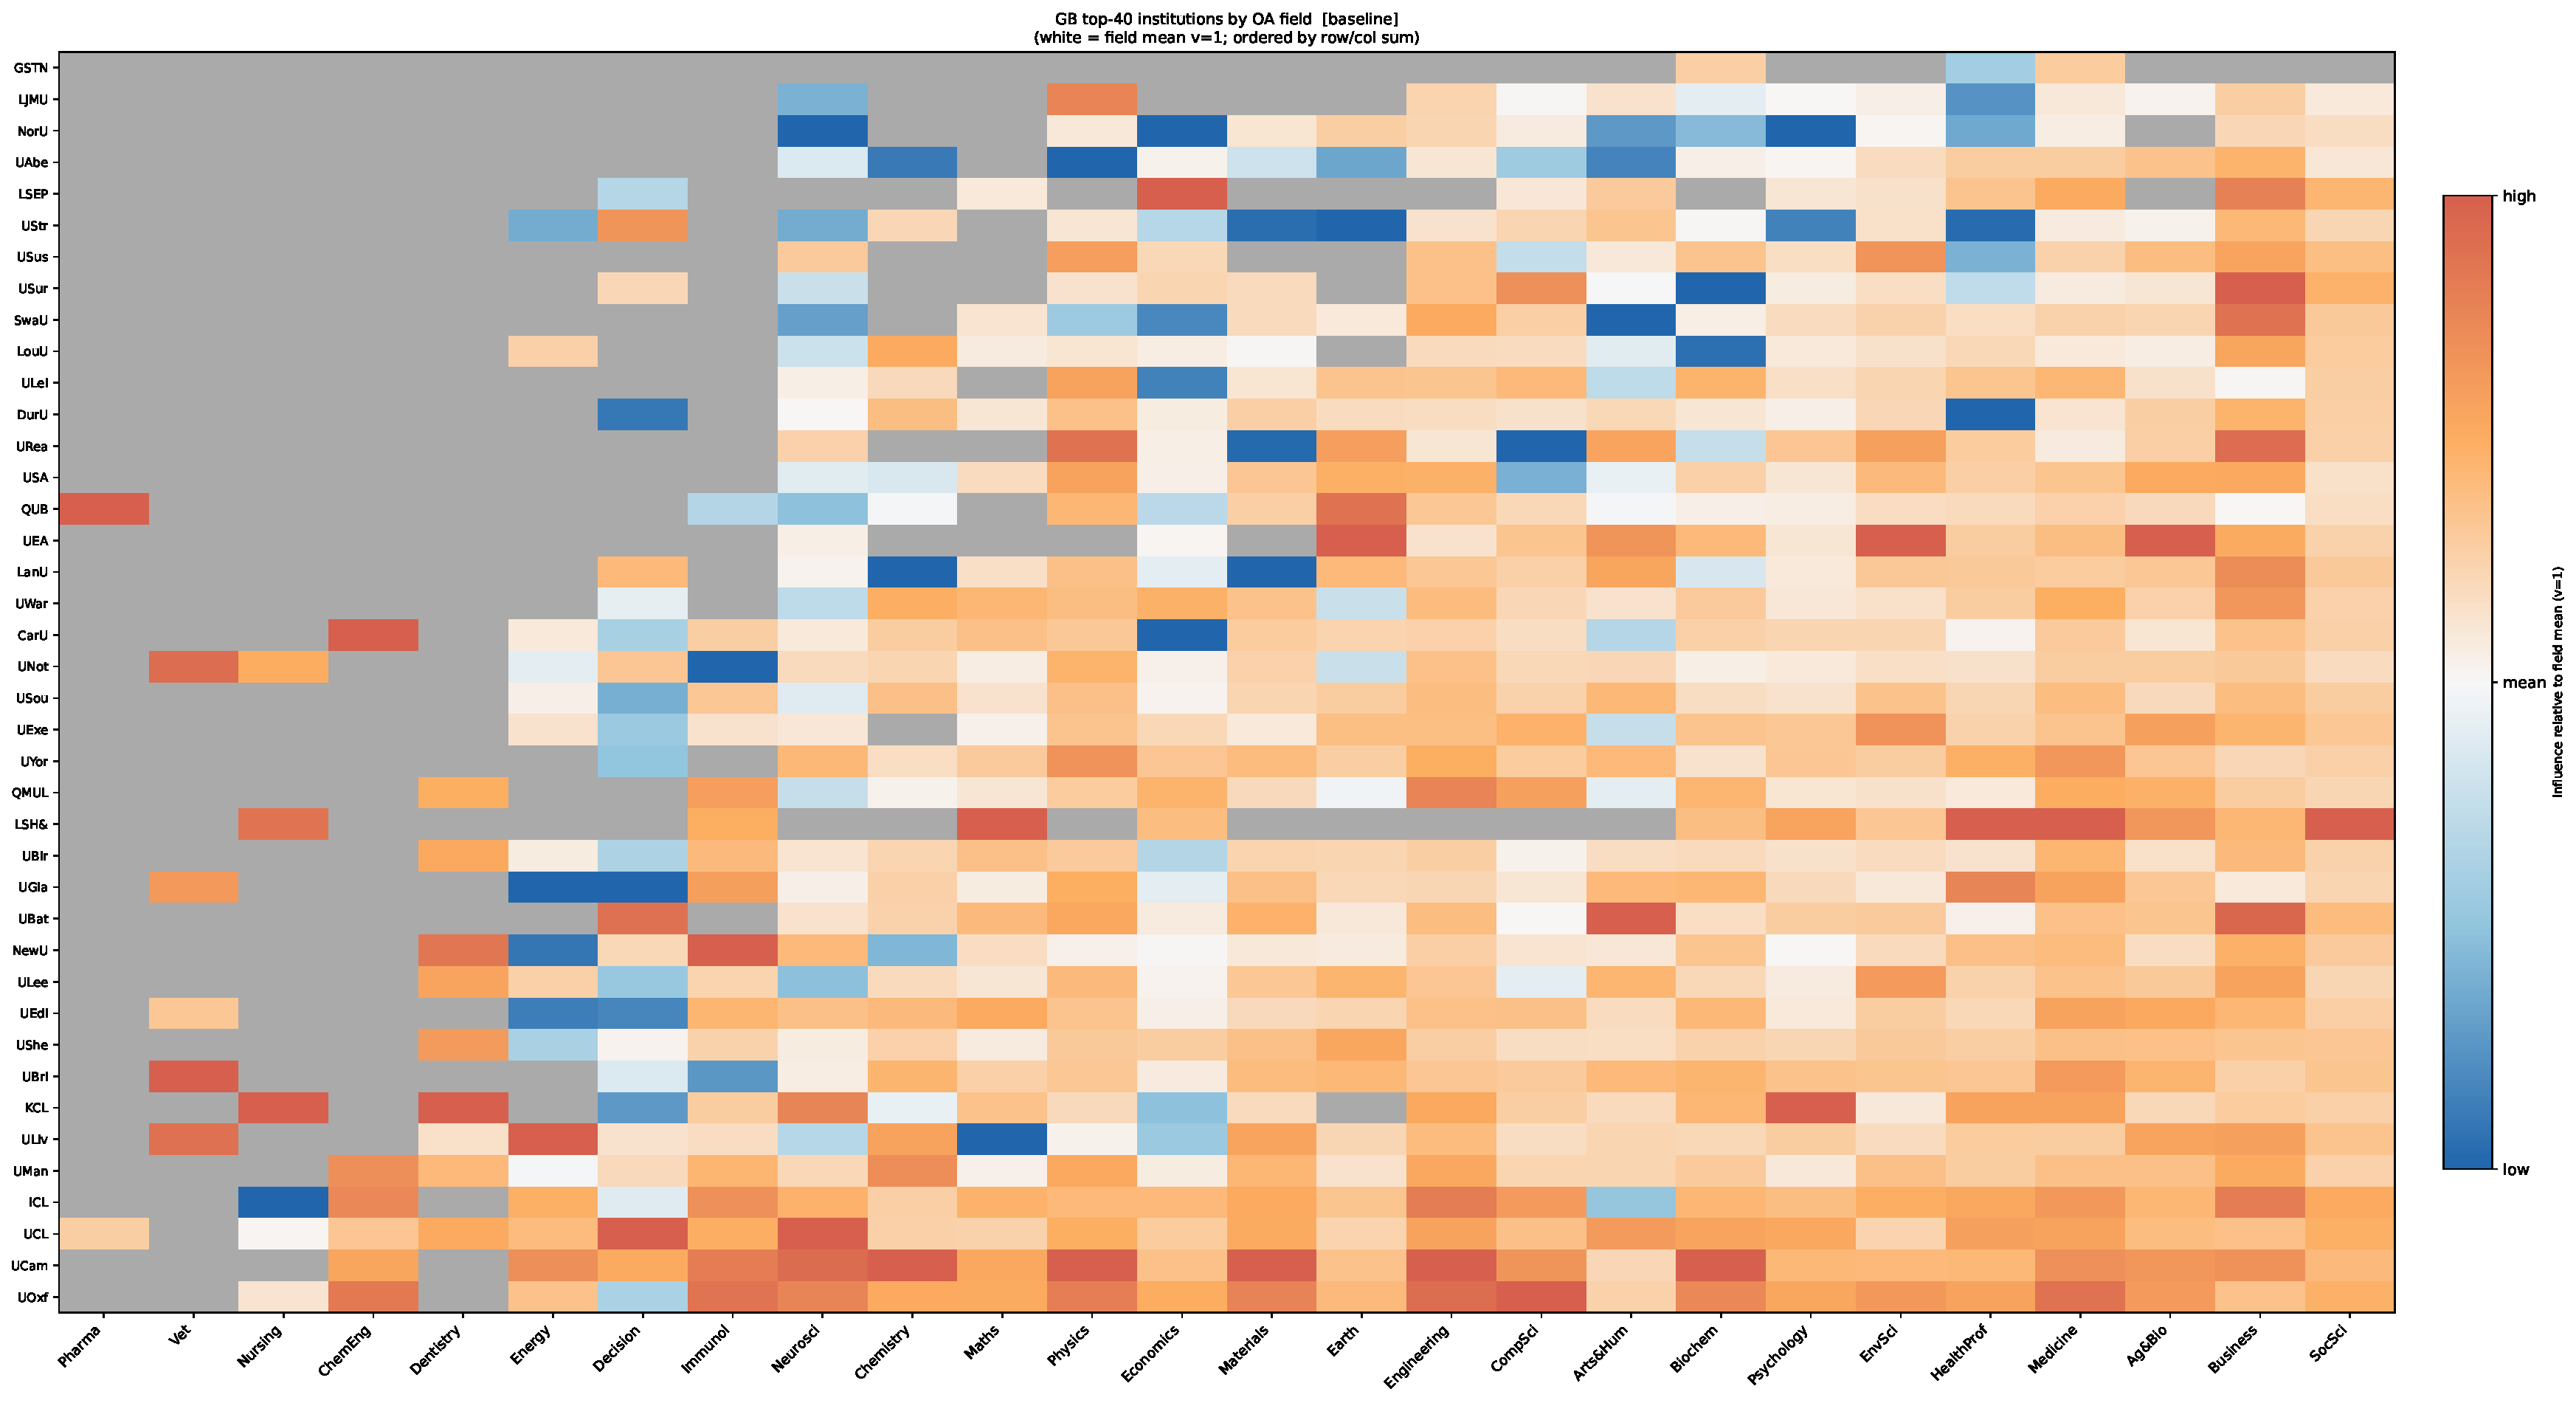
\includegraphics[width=\textwidth]{figures/fig3_country_heatmap_gb.pdf}
    \caption*{(b) United Kingdom (GB)}
\end{minipage}
\caption{Cross-country comparison of institutional research influence ($v_I$) across disciplines for top-ranked national universities in Australia and the United Kingdom.}
\label{fig:country_heatmap}
\end{figure}

The comparative profiles highlight a critical structural feature: unlike unipartite citation counts, which are inevitably dominated by large flagship multi-faculty campuses, bipartite prestige intensity illuminates specialized research institutes (e.g., medical research institutes and specialized polytechnics) with equal clarity across different national ecosystems.

\subsection{Algorithmic and Geopolitical Robustness}

A vital requirement for any national evaluation metric is stability against arbitrary boundary conditions and parameter specifications. We assess the resilience of the bipartite spectral ranking across two major dimensions: parameter perturbation and geopolitical citation bloc restriction.

Table~\ref{tab:sensitivity_correlations} reports the Spearman rank correlation ($\rho_s$) between baseline institutional rankings and five systematic variants across the five broad disciplines.

\begin{table}[htbp]
\centering
\small
\caption{Algorithmic and Geopolitical Stability: Spearman Rank Correlation ($\rho_s$) of Institutional Influence ($v_I$) between Baseline and Variants across the Five Broad Disciplines.}
\label{tab:sensitivity_correlations}
\begin{tabularx}{\textwidth}{>{\raggedright\arraybackslash}X ccccc}
\toprule
\textbf{Model / Bloc Variant} & \textbf{MCS} & \textbf{PSE} & \textbf{LES} & \textbf{BHS} & \textbf{SSH} \\
\midrule
OECD+G20 Bloc & 0.985 & 0.985 & 0.990 & 0.989 & 0.992 \\
OECD+G20 excl. CN/IN/US & 0.941 & 0.903 & 0.960 & 0.953 & 0.976 \\
AU, CN, IN, US Only & 0.956 & 0.949 & 0.942 & 0.935 & 0.017 \\
Retention Threshold ($\tau=20$) & 0.993 & 0.998 & 0.998 & 0.999 & 0.994 \\
Full Citation Count ($\rho=1$) & 0.953 & 0.908 & 0.966 & 0.973 & 0.975 \\
Sentinel Model ($\epsilon=1$) & 0.817 & 0.732 & 0.760 & 0.562 & 0.833 \\
\bottomrule
\end{tabularx}
\end{table}


\begin{figure}[htbp]
\centering
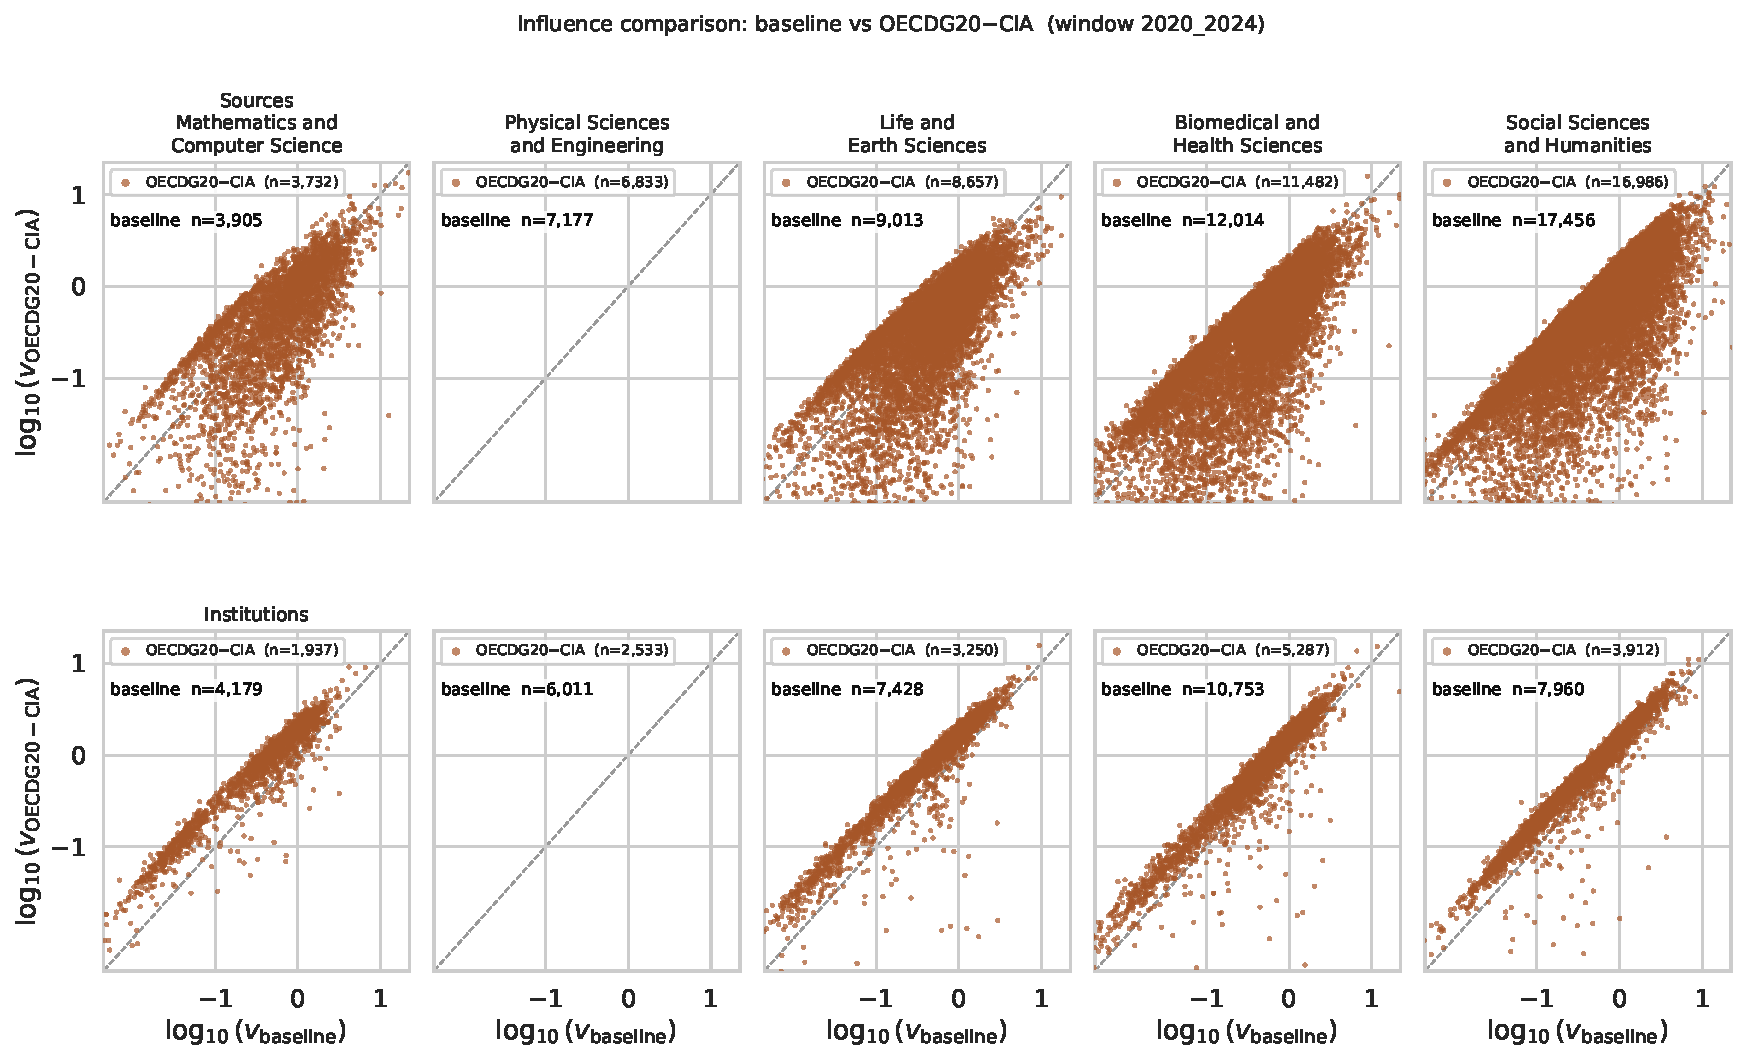
\includegraphics[width=0.88\textwidth]{figures/fig4_leiden_oecdg20cia_influence.pdf}
\caption{Stability of institutional influence ($v_I$) under geopolitical citation restriction: baseline global ranking ($x$-axis) versus the OECD+G20 excluding China, India, and the United States ($y$-axis) across sources (upper) and institutions (lower) for the five broad disciplines. The diagonal line denotes perfect invariance.}
\label{fig:bloc_stability}
\end{figure}

The empirical diagnostics demonstrate remarkable robustness:
\begin{itemize}
    \item \textbf{Retention Threshold Invariance ($\tau = 20$)}: Doubling the qualification threshold from 10 to 20 weighted works per year produces virtually identical institutional rankings, with Spearman rank correlations exceeding $0.993$ across all five disciplines.
    \item \textbf{Citation Multiplicity Weighting ($\rho = 1$)}: Replacing fixed-count citation weighting ($\rho = 0$) with full raw citation counts ($\rho = 1$) yields rank correlations between $0.908$ and $0.975$, proving that the bipartite projection is not hypersensitive to citation density normalization.
    \item \textbf{Geopolitical Bloc Stability}: When citations are restricted exclusively to the OECD+G20 bloc, institutional rank correlations exceed $0.985$ across all disciplines. Even when the world's three largest publishing powers (China, India, and the United States) are simultaneously excluded from the citation network (OECDG20-CIA), the rank correlation remains above $0.903$ in STEM and $0.976$ in SSH. As visualized in Figure~\ref{fig:bloc_stability}, institutions align tightly along the diagonal identity axis.
\end{itemize}

An instructive exception appears in the CIAA variant (AU, CN, IN, US only) within Social Sciences and Humanities ($\rho_s = 0.017$). In SSH, Chinese and Indian domestic citation networks operate in distinct linguistic and localized paradigms; restricting the entire world to this 4-country bloc severs the European, Commonwealth, and Latin American citation exchanges that anchor global social science discourse. This divergence affirms that the model sensitively captures genuine sociological realities rather than imposing a monolithic mathematical artifact.
